\documentclass[10pt,a4paper]{article}
\usepackage[latin1]{inputenc}
\usepackage{amsmath}
\usepackage{amsfonts}
\usepackage{amssymb}
\begin{document}

\section*{Mesh Generation}
One of the major strengths of the finite element method is its ability to break down a problem on a global domain to a problem on individual, simpler elements that together constitute an approximation of the domain. As the complexity of the geometry of the problem domain increases, the need for automatic and reliable meshing procedures is evident. 

\begin{figure}[htb]
	\centering
    \includegraphics[width=0.9\textwidth]{figures/basic_rect_mesh}
    \caption{A very basic meshing procedure for trivial geometries. Simply perform a Delaunay triangulation on a regular grid of points.}
    \label{fig:basic_rect_mesh}
\end{figure}

Figure \ref{fig:basic_rect_mesh} illustrates a first attempt at a basic meshing procedure. Given a very simple domain, a regular grid of points are triangulated using Delaunay triangulation. This approach has some very obvious limitations. For one, it is not immediately clear how to deal with unions of geometric shapes which may exhibit local properties, such as density or electrical permittivity. Simply overlaying the geometries on top of the grid is likely to result in very ill-shaped triangles, which may be disastrous for convergence of the finite element method. From these observations we may formulate some goals for practical mesh algorithms:

\begin{itemize}
  \item Preserve boundaries of original geometries.
  \item Propagate local properties of geometry to elements in mesh.
  \item Generate meshes with well-shaped elements.
  \item Generate meshes with the minimum number of elements to adequately capture the geometry.
\end{itemize}

The last point is not of crucial importance for our work, but in many cases it is desirable to only generate triangles where needed, and instead take advantage of adaptive mesh refinement to constraint dense regions of mesh elements to parts of the domain where they are needed.

The Swiss army knife of mesh generation is the Delaunay triangulation. Given a set of points, it generates a triangulation of the convex hull of the points, with the property that no points are contained inside the circumcircle of any triangle. Note that for the purposes of this project, we are only concerned with 2D meshes. A useful extension is the Constrained Delaunay Triangulation, which is similar to Delaunay triangulation, but imposes constraints on which vertices in the triangulation must be connected by edges. A constrained Delaunay triangulation does not in general have the Delaunay property.

Since it's generally harder to reduce a fine mesh to a coarse mesh, most mesh generation algorithms iteratively refine a coarse starting mesh until certain quality metrics are fulfilled. This might for instance be a minimum angle or maximum edge length. While there are many approaches to mesh refinement, we have mainly looked at a variant of Ruppert's algorithm \cite{ruppert}. In particular, Shewchuk \cite{shewchuk} demonstrates that it can be formulated with a Constrained Delaunay Triangulation as input. The aforementioned papers demonstrate the algorithm in detail, so we will only discuss the main points. As Shewchuk points out, a very interesting feature of Ruppert's algorithm is that while it takes a constrained Delaunay triangulation as input, its output is in fact Delaunay. Essentially, the output of the algorithm has two crucial properties: it is Delaunay, which minimizes the minimum angle of the triangles, and the triangles have a certain quality given constraints on size and shape.

\subsection*{Ruppert's algorithm}
In the following, a \emph{segment} is a constrained edge in the input constrained Delaunay triangulation, and every segment consists of a set of \emph{subsegments} in the iteratively refined triangulation. Note in particular that the set of subsegments is a subset of the set of edges in the triangulation, and that every segment is also a subsegment. Recall also that the \emph{circumcenter} of a triangle is the center of the unique circle such that all three vertices of the triangle lie exactly on the circle boundary.

\theoremstyle{definition}
\begin{definition}{\textbf{Encroached subsegment}}
A subsegment is \emph{encroached} if a vertex of the triangulation is contained in its \emph{diametral circle}, which is the smallest circle that contains the subsegment.
\end{definition}

\begin{figure}[htb]
	\centering
    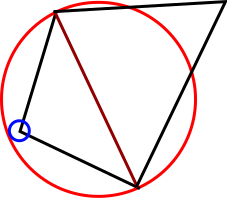
\includegraphics[width=0.6\textwidth]{figures/encroached}
    \caption{An example of an encroached subsegment. The dark red edge is a subsegment, the red circle its diametral circle and the vertex enclosed in the blue circle is a vertex that encroaches upon the subsegment.}
    \label{fig:encroached}
\end{figure}

It turns out that a constrained Delaunay triangulation without encroached subsegments is in fact Delaunay \cite{shewchuk}. Given the two output goals of Delaunay and triangle quality, the main idea of Ruppert's algorithm is to iteratively split any encroached subsegments until none remain, before it attempts to insert the circumcenters of ill-shaped triangles into the triangulation.

Figure \ref{fig:encroached} illustrates an encroached subsegment. A coarse outline of the algorithm follows. Note that when a point is inserted into the triangulation, an incremental Delaunay refinement algorithm is performed locally to compute the resulting triangulation.

\begin{algorithm}{\textbf{Ruppert's algorithm} (outline)}
\begin{enumerate}
	\item For any encroached subsegment, insert a vertex on its midpoint into the 	triangulation, effectively splitting the subsegment into two subsegments.
	\item Repeat the previous step until no subsegments are encroached.
	\item Consider a single poorly shaped triangle. If its circumcenter encroaches upon any subsegments, split the subsegments. Otherwise, insert the circumcenter into the triangulation.
	\item Repeat the algorithm from step 1 until there are no encroached edges and no poorly shaped triangles.
\end{enumerate}
\end{algorithm}

In \cite{ruppert}, Ruppert proves that given certain bounds on the angles of the input constraints, the algorithm terminates for a maximum angle of $20 \degree$, though he notes that in practice you are able to select larger values up to $\approx 30 \degree$. In \cite{shewchuk} it is claimed that the angles of the constrained segments in the input graph must be larger than $60 \degree$ to guarantee termination.

For practical purposes, such bounds on the input are not realistic, and so practical implementations must guarantee termination in the face of badly shaped input data. Some practical algorithms for deciding when to terminate are found in \cite{5}. A more recent and arguably better approach was introduced by Miller-Pav-Walkington in \cite{miller}.




\end{document}